\documentclass[../../main.tex]{subfiles}
\graphicspath{{../../image/}{../../figure/}}
\begin{document}

\section{连续流}\label{section:ch18-连续流}

本章将要探讨的最后一种标准化流采用了常微分方程（Ordinary Differential Equation, ODE）定义的深度神经网络，它可以看成具有无限多层数的深层网络。我们首先介绍神经常微分方程（简称神经 ODE）的概念，然后将其应用于标准化流模型的构建。

神经网络包含的处理层越多，神经网络就越有用，我们不妨探究一下，如果层数无限多会发生什么。考虑一个残差网络，其中每一层生成的输出由输入向量加上该输入向量的某个参数化非线性函数给出：
\begin{align}
z(t+1)=z(t)+f\big(z(t),w\big)
\label{align:ch18-residual}
\end{align}
其中 $t=1,\cdots,T$ 标记了网络中的层。注意，我们在每一层都使用了相同的函数，并且共享参数向量 $w$，因为这允许我们在参数数量有限的情况下考虑任意多的层。想象一下，增加层数，同时确保在每一层引入的变化相应地变得更小。在极限情况下，隐藏单元激活向量变成了连续变量 $t$ 的函数 $z(t)$，我们可以将这个向量通过网络的演化表示为一个微分方程（见习题 18.5）：
\begin{align}
\frac{\mathrm{d}z(t)}{\mathrm{d}t}=f\big(z(t),w\big)
\label{align:ch18-neural-ode}
\end{align}
其中 $t$ 通常称为``时间''。式~\eqref{align:ch18-neural-ode} 所示的方程就称为\textbf{神经 ODE}（Chen et al., 2018）。常微分方程的``常''指的是只有单一变量 $t$。如果将网络的输入表示为向量 $z(0)$，则输出 $z(T)$ 可以通过积分微分方程来获得：
\begin{align}
z(T)=z(0)+\int_{0}^{T}f\big(z(t),w\big)\,\mathrm{d}t
\label{align:ch18-ode-integral}
\end{align}
这个积分可以使用标准数值积分软件工具来计算。求解微分方程最简单的方法是欧拉前向积分法（forward integration），对应于式~\eqref{align:ch18-residual}。在实际操作中，更强大的数值积分算法可以通过调整其函数计算来实现目标。特别是，它们可以自适应地选择通常为非均匀分布的 $t$ 的值。这种计算次数取代了传统分层网络中``深度''的概念。传统分层网络与神经 ODE 的比较如图~\ref{fig:ch18-ode-compare} 所示。

\begin{figure}[htbp]
\centering
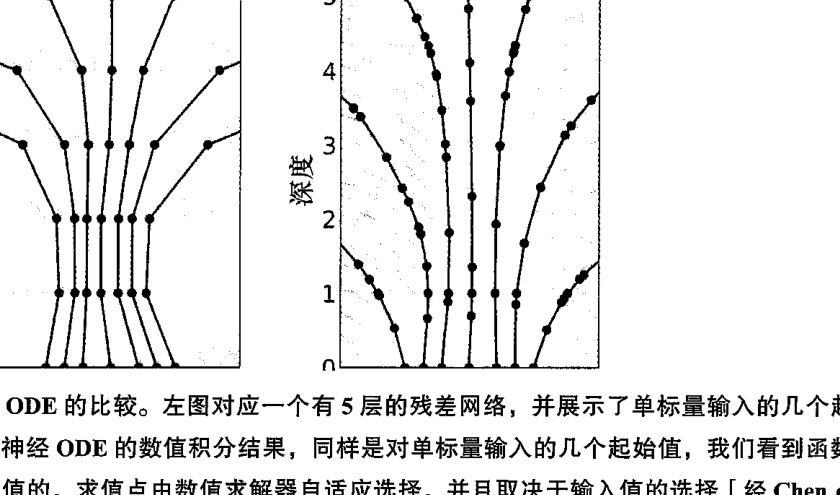
\includegraphics[width=0.85\textwidth]{ch18-fig503-ode-compare.png}
\caption{传统分层网络与神经 ODE 的比较。左图对应一个有 $5$ 层的残差网络，展示了单标量输入的几个起始值的轨迹；右图显示了连续神经 ODE 的数值积分结果，同样是对单标量输入的几个起始值，求值点由数值求解器自适应选择，并且取决于输入值的选择（Chen et al., 2018，经授权使用）。}
\label{fig:ch18-ode-compare}
\end{figure}

\subsection{神经 ODE 的反向传播}\label{subsection:ch18-ode-backprop}

我们现在需要解决如何训练神经 ODE 的问题，即如何通过优化损失函数来确定 $w$ 的值。给定一个数据集，其中包括输入向量 $z(0)$ 的值以及相关的输出目标向量，以及一个依赖于输出向量 $z(T)$ 的损失函数 $L(\cdot)$。一种方法是使用自动微分来微分 ODE 求解器在前向传播期间执行的所有操作（参见 8.2 节）。尽管这样做很直接，但从内存角度来看却代价高昂，并且在控制数值误差方面也不是最佳做法。另一种方法（Chen et al., 2018）将 ODE 求解器视为一个黑箱，并使用了一种称为\textbf{伴随灵敏度方法}（adjoint sensitivity method）的技术，这可以视为显式反向传播的连续类比。

回想一下，反向传播涉及对每个数据点执行三个连续操作步骤（参见第 8 章）：前向传播，计算网络中每一层的激活向量；反向传播，从输出层开始利用微积分的链式法则计算损失函数对每一层激活的导数，并向后传播；参数梯度计算，通过将前向传播的激活值和反向传播的梯度相乘来计算损失函数对网络参数的导数。

为了将反向传播应用于神经 ODE，定义一个称为\textbf{伴随}（adjoint）的量（见习题 18.6）：
\begin{align}
a(t)=\frac{\partial L}{\partial z(t)}
\label{align:ch18-adjoint}
\end{align}
$a(T)$ 对应于损失函数关于输出向量的常规导数。$a(t)$ 满足如下微分方程：
\begin{align}
\frac{\mathrm{d}a(t)}{\mathrm{d}t}=-a(t)^{\mathsf T}\,\nabla_{z}f\big(z(t),w\big)
\label{align:ch18-adjoint-ode}
\end{align}
这是微积分链式法则的连续版本。这可以通过从 $a(T)$ 开始向后积分来求解，并且在计算神经 ODE 的梯度时可以执行类似的步骤。

反向传播的第三步通过计算激活值和梯度的适当乘积来计算损失函数对网络参数的导数。当一个网络中的多个连接共享一个参数值时，总导数由每个连接的导数相加而成（见习题 9.7）。对于神经 ODE，其中相同的参数向量 $w$ 在整个网络中共享，求和变成了对 $t$ 的积分，形式如下（见习题 18.7）：
\begin{align}
\nabla_{w}L=-\int_{0}^{T}a(t)^{\mathsf T}\,\nabla_{w}f\big(z(t),w\big)\,\mathrm{d}t
\label{align:ch18-param-grad}
\end{align}
式~\eqref{align:ch18-adjoint-ode} 中的 $\nabla_{z}$ 和式~\eqref{align:ch18-param-grad} 中的 $\nabla_{w}$ 可以使用自动微分高效地求值（见 8.2 节）。注意，上述结果同样适用于更普遍的神经网络函数 $f(z(t),t,w)$，它除了通过 $z(t)$ 的隐式依赖之外，还显式地依赖于 $t$。

与传统分层网络相比，使用伴随方法训练的神经 ODE 的一个好处是，不需要存储前向传播的中间结果，因此内存成本是恒定的。此外，神经 ODE 可以自然地处理连续时间数据，其中观测可在任意时间发生。如果损失函数 $L$ 依赖于 $z(T)$ 的其他值而不仅仅是输出值，则需要进行多次逆模型求解，对每一对连续的输出进行一次逆模型求解，以便单个解决方案可以分解为多个连续解决方案以访问中间状态。请注意，在训练阶段可以使用高精度的求解器；而在推理阶段，特别是在计算资源有限的应用场景中，可以采用较低的精度，从而减少所需的函数评估次数。

\end{document}